%% Creator: Inkscape inkscape 0.92.1, www.inkscape.org
%% PDF/EPS/PS + LaTeX output extension by Johan Engelen, 2010
%% Accompanies image file 'e_N_m_r.pdf' (pdf, eps, ps)
%%
%% To include the image in your LaTeX document, write
%%   \input{<filename>.pdf_tex}
%%  instead of
%%   \includegraphics{<filename>.pdf}
%% To scale the image, write
%%   \def\svgwidth{<desired width>}
%%   \input{<filename>.pdf_tex}
%%  instead of
%%   \includegraphics[width=<desired width>]{<filename>.pdf}
%%
%% Images with a different path to the parent latex file can
%% be accessed with the `import' package (which may need to be
%% installed) using
%%   \usepackage{import}
%% in the preamble, and then including the image with
%%   \import{<path to file>}{<filename>.pdf_tex}
%% Alternatively, one can specify
%%   \graphicspath{{<path to file>/}}
%% 
%% For more information, please see info/svg-inkscape on CTAN:
%%   http://tug.ctan.org/tex-archive/info/svg-inkscape
%%
\begingroup%
  \makeatletter%
  \providecommand\color[2][]{%
    \errmessage{(Inkscape) Color is used for the text in Inkscape, but the package 'color.sty' is not loaded}%
    \renewcommand\color[2][]{}%
  }%
  \providecommand\transparent[1]{%
    \errmessage{(Inkscape) Transparency is used (non-zero) for the text in Inkscape, but the package 'transparent.sty' is not loaded}%
    \renewcommand\transparent[1]{}%
  }%
  \providecommand\rotatebox[2]{#2}%
  \ifx\svgwidth\undefined%
    \setlength{\unitlength}{655.22437106bp}%
    \ifx\svgscale\undefined%
      \relax%
    \else%
      \setlength{\unitlength}{\unitlength * \real{\svgscale}}%
    \fi%
  \else%
    \setlength{\unitlength}{\svgwidth}%
  \fi%
  \global\let\svgwidth\undefined%
  \global\let\svgscale\undefined%
  \makeatother%
  \begin{picture}(1,0.49764391)%
    \put(0,0){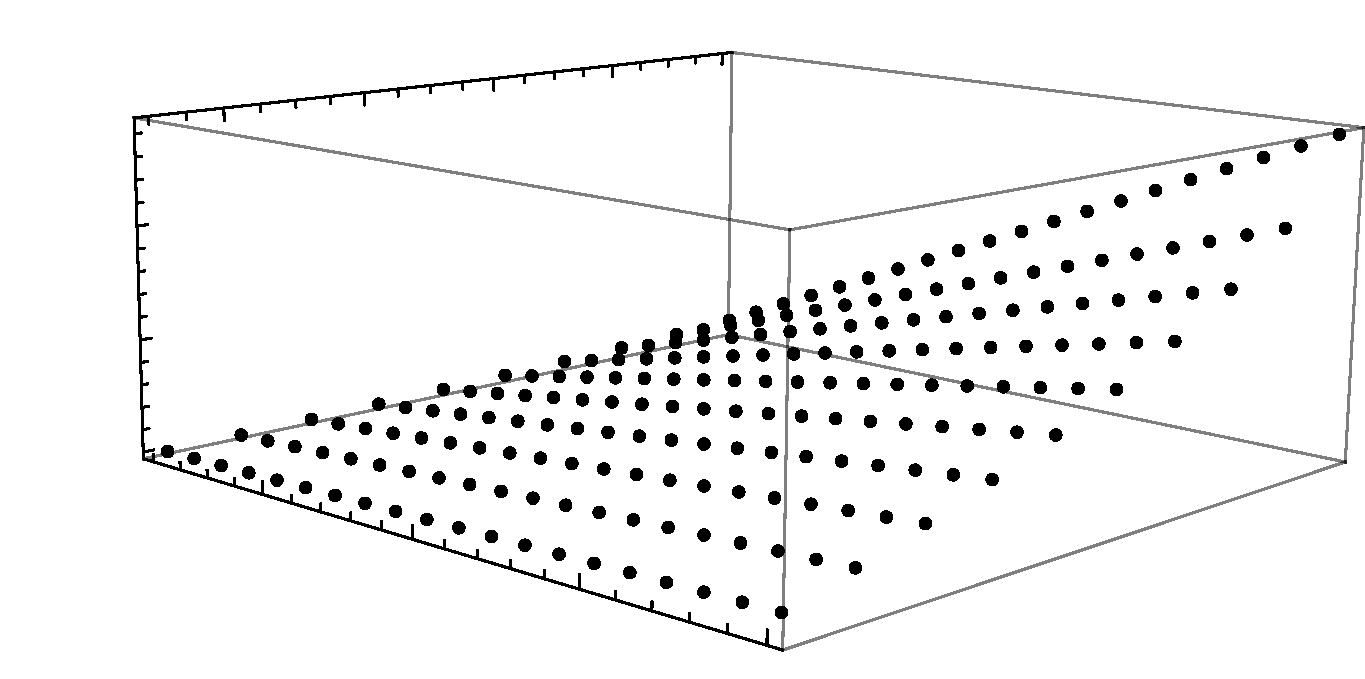
\includegraphics[width=\unitlength,page=1]{e_N_m_r.pdf}}%
    \put(0.02005506,0.26499131){\color[rgb]{0,0,0}\makebox(0,0)[lb]{\smash{}}}%
    \put(0.07731963,0.15947698){\color[rgb]{0,0,0}\makebox(0,0)[lb]{\smash{0}}}%
    \put(0.04277064,0.39382041){\color[rgb]{0,0,0}\makebox(0,0)[lb]{\smash{2800}}}%
    \put(0.04569407,0.24329679){\color[rgb]{0,0,0}\makebox(0,0)[lb]{\smash{1000}}}%
    \put(0.04372186,0.32514434){\color[rgb]{0,0,0}\makebox(0,0)[lb]{\smash{2000}}}%
    \put(0.15767762,0.11139749){\color[rgb]{0,0,0}\rotatebox{13.620502}{\makebox(0,0)[lb]{\smash{500}}}}%
    \put(0.25577773,0.07760436){\color[rgb]{0,0,0}\rotatebox{13.620502}{\makebox(0,0)[lb]{\smash{1000}}}}%
    \put(0.37596744,0.04142163){\color[rgb]{0,0,0}\rotatebox{13.620502}{\makebox(0,0)[lb]{\smash{1500}}}}%
    \put(0.51482739,-0.00031079){\color[rgb]{0,0,0}\rotatebox{13.620502}{\makebox(0,0)[lb]{\smash{2000}}}}%
    \put(0.29736576,0.48848749){\color[rgb]{0,0,0}\makebox(0,0)[lb]{\smash{r}}}%
    \put(0.22812538,0.04804597){\color[rgb]{0,0,0}\makebox(0,0)[lb]{\smash{m}}}%
    \put(-0.00163947,0.28569974){\color[rgb]{0,0,0}\makebox(0,0)[lb]{\smash{E[N]}}}%
    \put(0.15022228,0.43425114){\color[rgb]{0,0,0}\makebox(0,0)[lb]{\smash{0.2}}}%
    \put(0.25281321,0.44481629){\color[rgb]{0,0,0}\makebox(0,0)[lb]{\smash{0.4}}}%
    \put(0.34783228,0.45601554){\color[rgb]{0,0,0}\makebox(0,0)[lb]{\smash{0.6}}}%
    \put(0.43390644,0.46489058){\color[rgb]{0,0,0}\makebox(0,0)[lb]{\smash{0.8}}}%
    \put(0.51385156,0.47309656){\color[rgb]{0,0,0}\makebox(0,0)[lb]{\smash{1.0}}}%
  \end{picture}%
\endgroup%
